%作者:汪斐然
%模板用途:模式识别报告
%时间:2021年3月

%这是一份基于《2020-2021模式识别期末提交模板》Word版制作的Latex模板。用于方昱春老师的模式识别课程报告。
%文档中对Latex的各种使用方式都准备了样例并进行备注,包括标题设置、图表添加、文献引用以及字体设置等。
%参考文献格式和Word版存在一定的区别,使用的是IEEETR格式。是IEEE期刊使用的参考文献引用标准。
%参考文献选择使用IEEETR格式的原因在于,可以在文章中对参考文献进行超链接索引。
%希望这份模板可以帮助同学们快速上手Latex,制作漂亮的课程报告;可以在同学们之后的研究学习过程中成为学术论文的参考模板。

%Latex工具:本地编辑平台:TexWorks;在线编辑平台:Overleaf(推荐)

%Latex快速入门教程:
%1、https://muyuuuu.github.io/2018/11/07/Brief-introduction-to-LaTex/
%2、https://liam.page/2014/09/08/latex-introduction/

%Latex快速辅助工具使用说明:
%快速绘制表格工具:https://www.tablesgenerator.com/
%快速生成公式工具:https://mathpix.com/

%%%%%%%%%%%%%%%%%%%%%%%%%%%%%环境配置%%%%%%%%%%%%%%%%%%%%%%%%%%%%%%%%%%

\documentclass{article}
\usepackage[UTF8]{ctex}
\usepackage[left=3.18cm,right=3.18cm,top=2.54cm,bottom=2.54cm]{geometry}
\geometry{a4paper}

%附录包
\usepackage{appendix} 
\usepackage{listings}

%代码格式
\usepackage{xcolor}
\lstset{
    numbers=left, 
    numberstyle= \tiny, 
    keywordstyle= \color{ blue!70},
    commentstyle= \color{red!50!green!50!blue!50}, 
    frame=shadowbox, % 阴影效果
    rulesepcolor= \color{ red!20!green!20!blue!20} ,
    escapeinside=``, % 英文分号中可写入中文
    xleftmargin=2em,xrightmargin=2em, aboveskip=1em,
    framexleftmargin=2em
} 
\usepackage{algorithm}
\usepackage{algpseudocode}
\renewcommand{\algorithmicrequire}{\textbf{Input:}}  % Use Input in the 
\renewcommand{\algorithmicensure}{\textbf{Output:}} % Use Output in the 

%数学
\usepackage{amsmath}
\usepackage{amsthm}

%图片
\usepackage{graphicx} %添加图片

%字体、格式设置
\usepackage{subfigure}
\usepackage{float}
\usepackage{xeCJK}
\renewcommand{\vec}[1]{\boldsymbol{#1}} % 生产粗体向量,而不是带箭头的向量
\usepackage{amssymb}
\usepackage{booktabs} % excel导出的大表格
\usepackage{hyperref}
\usepackage{titlesec}%设置字体的包
\usepackage{multirow}
%可选字体:
% \noindent 中文字体(默认宋体)\\
% \fangsong 中文字体(仿宋) \songti 中文字体(宋体) \lishu 中文字体(隶书) \heiti 中文字体(黑体)\\
% \CJKfamily{zhkai} 中文字体(楷书) \CJKfamily{zhyou} 中文字体(幼圆) \CJKfamily{zhyahei} 中文字体(微软雅黑)\\

%调整图表标题的字体样式
\usepackage{caption}
\captionsetup{font={small,bf}} 

%新定义
\newtheorem{definition}{定义} %中文
\newtheorem{lemma}{引理}
\newtheorem{theorem}{定理}
\DeclareMathOperator{\Ima}{Im}%定义新符号
\DeclareMathOperator{\Rank}{rank}%定义求秩算子



%设置标题,作者
\title{\textbf{基于卷积神经网络与SVM的路标识别}}
\author{
郑力铖(21122873)
}

%%%%%%%%%%%%%%%%%%%%%%%%%%%%%%%正文%%%%%%%%%%%%%%%%%%%%%%%%%%%%%%%%%%
%\songti(宋体)设置全文字体,可改为\heiti(黑体),\fangsong(仿宋)
\begin{document} \songti

% 插入封面
\centerline{\heiti\zihao{2}{上海大学2023 $ \sim $ 2024学年}}
\vspace{10bp}
\centerline{\heiti\zihao{2}{课程报告成绩评价表}}

\vskip 2cm

\begin{flushleft}
    \zihao{3}
    {\heiti{课程名称:}}
    {\heiti\underline{\quad\textbf{《模式识别》}\quad}}
    {\heiti{课程编号:}}
    {\heiti\underline{\quad\textbf{08306089}\hspace{1cm}}}  \\
    \vspace{20bp}
    {\heiti{ {报告名称:}}}
    {\heiti\underline{\quad\textbf{基于HOG+SVM与YOLO的路标识别}\quad}} \\
    \vspace{20bp}
    {\heiti{{姓}\quad\quad{名:}}}
    {\heiti\underline{\quad\quad\textbf{郑力铖}\quad\quad}}
    {\heiti{{学}\quad\quad{号:}}}
    {\heiti\underline{\quad\textbf{21122873}\quad}} \\
    \vspace{20bp}
    {\heiti{ {报告评语:}}} \\
    \vspace{5bp}
    \fbox{
        \parbox{\textwidth}{
            \begin{center}
                \leavevmode \\ \quad
                \leavevmode \\ \quad
                \leavevmode \\ \quad
                \leavevmode \\ \quad
            \end{center}
        }
    }

    \vspace{20bp}
    {\heiti{{报告成绩:}}}
    \\
    \vspace{5bp}
    \begin{table}[htbp]
        \setlength{\tabcolsep}{0.37cm}{
            \begin{tabular}{|cl|cl|cll|c|}
                \hline
                \multicolumn{2}{|c|}{方案设计(20分)}          & \multicolumn{2}{c|}{验收(20分)}              & \multicolumn{3}{c|}{书面报告(60分)}          & \multirow{2}{*}{总分}                                                                                                                                                                                                     \\ \cline{1-7}
                \multicolumn{1}{|c|}{\begin{tabular}[c]{@{}c@{}}可行性\\ (10分)\end{tabular}} & \multicolumn{1}{c|}{\begin{tabular}[c]{@{}c@{}}创新性\\ (10分)\end{tabular}} & \multicolumn{1}{c|}{\begin{tabular}[c]{@{}c@{}}规范性\\ (10分)\end{tabular}} & \multicolumn{1}{c|}{\begin{tabular}[c]{@{}c@{}}演示效果\\ (10分)\end{tabular}} & \multicolumn{1}{c|}{\begin{tabular}[c]{@{}c@{}}规范性\\ (20分)\end{tabular}} & \multicolumn{1}{c|}{\begin{tabular}[c]{@{}c@{}}完整性\\ (20分)\end{tabular}} & \multicolumn{1}{c|}{\begin{tabular}[c]{@{}c@{}}科学性\\ (20分)\end{tabular}} &                       \\ \hline
                \multicolumn{1}{|l|}{}                          &                                                & \multicolumn{1}{l|}{}                          &                                                & \multicolumn{1}{l|}{}                          & \multicolumn{1}{l|}{}                          &                                                & \multicolumn{1}{l|}{} \\ \hline
            \end{tabular}}
    \end{table}
\end{flushleft}

\vspace{20bp}
\leftline{\heiti\zihao{3}{任课教师:}}
\vspace{20bp}
\leftline{\heiti\zihao{3} {评阅日期:     \quad\quad\quad     年  \quad\quad  月  \quad\quad  日         }} %调用封面文件

\date{}
\maketitle


%%%%%%%%%%%%%%%%%%%%%%摘要%%%%%%%%%%%%%%%%%%%%%%%%%%%%%
%由摘要和关键词两部分组成
\begin{center}
    \setlength{\textwidth}{15cm}
    \parbox{\textwidth}{
        \textbf{摘要:}作为交通系统的基本要素,交通标志提供了关于驾驶员、行人等的道路状况的重要信息,来降低事故风险。随着计算机视觉和人工智能的快速发展,交通标志识别算法已被应用于先进的驾驶员辅助系统和自动驾驶系统,以帮助驾驶员和自动驾驶车辆准确获取道路信息。然而在实际应用中,交通标志识别仍然具有挑战性。本文对比了经典的机器学习方法HOG+SVM,和通用视觉识别模型yolov5和yolov8方法,探讨在自动驾驶场景下的路标识别方法。
        \newline
        \textbf{关键词:}图像识别, 支持向量机, 深度学习, 神经网络。
    }
\end{center}

%%%%%%%%%%%%%%%%%%%%%%目录%%%%%%%%%%%%%%%%%%%%%%%%%%%%%
% \newpage
% \tableofcontents
% \newpage
%%%%%%%%%%%%%%%%%%%%%%%%%%%%%%%%%%%%%%%%%%%%%%%%%%%%%%%%
%一级标题
\section{引言}
%%%%%%%%%%%%%%%%%%%%%%%%%%%
%二级标题
\subsection{提出问题(300-500字)}
%三级标题
\subsubsection{三级标题}
正文正文正文正文正文正文正文正文正文正文,正文正文正文正文正文正文正文正文正文正文。正文正文正文正文正文正文正文正文正文正文正文,正文正文正文正文正文正文正文正文正文正文。正文正文正文正文正文正文正文正文正文正文正文,正文正文正文正文正文正文正文正文正文正文。

\subsubsection{三级标题}
正文正文正文正文正文正文正文正文正文正文,正文正文正文正文正文正文正文正文正文正文。正文正文正文正文正文正文正文正文正文正文正文,正文正文正文正文正文正文正文正文正文正文。正文正文正文正文正文正文正文正文正文正文正文,正文正文正文正文正文正文正文正文正文正文。

%%%%%%%%%%%%%%%%%%%%%%%%%%%
\subsection{求解方案分析}
早在 2005 年,方向梯度直方图(HOG)就被提出,HOG用来提取图片特征,并和支持向量机(SVM)结合,进行行人检测。HOG+SVM这种经典的机器学习方法在过去取得了一定的成功,但随着技术的进步,人们开始寻求更加高效、准确的解决方案。

近年来,YOLO算法以其高速度和高精度迅速走红。

因此,本文深入研究了yolov5和yolov8这两种先进的目标检测模型。这两种模型都是基于yolo模型的优化,利用深度学习技术,通过神经网络层次结构和先进的目标检测算法,在图像中快速准确地识别路标。相较于传统方法,它们在处理复杂场景和多类别标识时表现更为出色。

在自动驾驶场景下,路标识别至关重要。本文通过对比这些方法的实际应用效果,旨在为自动驾驶系统选择最合适的路标识别方法提供参考。考虑到实时性、准确性和鲁棒性等因素,读者将能够更好地了解何种方法在特定条件下更为适用。

%%%%%%%%%%%%%%%%%%%%%%%%%%%
\subsection{论文概述(200字)}
正文正文正文正文正文正文正文正文正文正文,正文正文正文正文正文正文正文正文正文正文。正文正文正文正文正文正文正文正文正文正文正文,正文正文正文正文正文正文正文正文正文正文。正文正文正文正文正文正文正文正文正文正文正文,正文正文正文正文正文正文正文正文正文正文。

%%%%%%%%%%%%%%%%%%%%%%%%%%%%%%%%%%%%%%%%%%%%%%%%%%%%%%%%
\section{相关算法概述}
%%%%%%%%%%%%%%%%%%%%%%%%%%%
\subsection{梯度直方图与支持向量机(HOG+SVM)}
正文正文正文正文正文正文正文正文正文正文,正文正文正文正文正文正文正文正文正文正文。正文正文正文正文正文正文正文正文正文正文正文,正文正文正文正文正文正文正文正文正文正文。正文正文正文正文正文正文正文正文正文正文正文,正文正文正文正文正文正文正文正文正文正文,如图\ref{fig:sample}所示。
\begin{figure}[H]
    \centering
    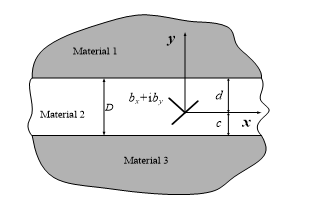
\includegraphics[width=0.5\textwidth]{sample.png}
    \caption{位于三层材料体系中的位错示意图}
    \label{fig:sample}
\end{figure}

\subsection{对象检测算法YOLO}
YOLO(You Only Look Once)是一种流行的对象检测和图像分割模型,由华盛顿大学的Joseph Redmon和Ali Farhadi开发。


%%%%%%%%%%%%%%%%%%%%%%%%%%%%%%%%%%%%%%%%%%%%%%%%%%%%%%%%
\section{算法实现描述}
正文正文正文正文正文正文正文正文正文正文,正文正文正文正文正文正文正文正文正文正文。正文正文正文正文正文正文正文正文正文正文正文,正文正文正文正文正文正文正文正文正文正文。正文正文正文正文正文正文正文正文正文正文正文,正文正文正文正文正文正文正文正文正文正文。

\subsection{算法总体框架(>500字)}
正文正文正文正文正文正文正文正文正文正文,正文正文正文正文正文正文正文正文正文正文。正文正文正文正文正文正文正文正文正文正文正文,正文正文正文正文正文正文正文正文正文正文。正文正文正文正文正文正文正文正文正文正文正文,正文正文正文正文正文正文正文正文正文正文,引用参考文献\cite{HSV}。


\subsection{改进一及分析(>500字)}
正文正文正文正文正文正文正文正文正文正文,正文正文正文正文正文正文正文正文正文正文。正文正文正文正文正文正文正文正文正文正文正文,正文正文正文正文正文正文正文正文正文正文。正文正文正文正文正文正文正文正文正文正文正文,正文正文正文正文正文正文正文正文正文正文,引用参考文献\cite{ml}。

\subsection{改进二及分析(>500字)}
正文正文正文正文正文正文正文正文正文正文,正文正文正文正文正文正文正文正文正文正文。正文正文正文正文正文正文正文正文正文正文正文,正文正文正文正文正文正文正文正文正文正文。正文正文正文正文正文正文正文正文正文正文正文,正文正文正文正文正文正文正文正文正文正文\cite{imgaug}。


%%%%%%%%%%%%%%%%%%%%%%%%%%%%%%%%%%%%%%%%%%%%%%%%%%%%%%%%
\section{实验描述}
\subsection{实验数据和实验方案 (>500字)}
正文正文正文正文正文正文正文正文正文正文,正文正文正文正文正文正文正文正文正文正文。正文正文正文正文正文正文正文正文正文正文正文,正文正文正文正文正文正文正文正文正文正文。正文正文正文正文正文正文正文正文正文正文正文,正文正文正文正文正文正文正文正文正文正文。

\subsection{实验一及结果分析 (>500字)}
正文正文正文正文正文正文正文正文正文正文,正文正文正文正文正文正文正文正文正文正文。正文正文正文正文正文正文正文正文正文正文正文,正文正文正文正文正文正文正文正文正文正文。正文正文正文正文正文正文正文正文正文正文正文,正文正文正文正文正文正文正文正文正文正文。

\subsection{实验二及结果分析 (>500字)}
正文正文正文正文正文正文正文正文正文正文,正文正文正文正文正文正文正文正文正文正文。正文正文正文正文正文正文正文正文正文正文正文,正文正文正文正文正文正文正文正文正文正文。正文正文正文正文正文正文正文正文正文正文正文,正文正文正文正文正文正文正文正文正文正文。

%%%%%%%%%%%%%%%%%%%%%%%%%%%%%%%%%%%%%%%%%%%%%%%%%%%%%%%%
\section{结论(500字)}
正文正文正文正文正文正文正文正文正文正文,正文正文正文正文正文正文正文正文正文正文。正文正文正文正文正文正文正文正文正文正文正文,正文正文正文正文正文正文正文正文正文正文。正文正文正文正文正文正文正文正文正文正文正文,正文正文正文正文正文正文正文正文正文正文。

%%%%%%%%%%%%%%%%%%%%%%%%%%%%%%%%%%%%%%%%%%%%%%%%%%%%%%%%
\section{学习体会和建议(300字)}
正文正文正文正文正文正文正文正文正文正文,正文正文正文正文正文正文正文正文正文正文。正文正文正文正文正文正文正文正文正文正文正文,正文正文正文正文正文正文正文正文正文正文。正文正文正文正文正文正文正文正文正文正文正文,正文正文正文正文正文正文正文正文正文正文。

%%%%%%%%%%%%%%%%%%%引用文献%%%%%%%%%%%%%%%%%%%%%%%%%%%%%%
\bibliography{article}      % 指定article 代表同目录下的article.bib文件 
\bibliographystyle{ieeetr}  % 定义文献引用的格式

%%%%%%%%%%%%%%%%%%%%%%%附录%%%%%%%%%%%%%%%%%%%%%%%%%%%%%%
\newpage{}
\appendix
\section{附录}
\begin{appendices}
    1、图模板
    \begin{figure}[htpb]
        \centering
        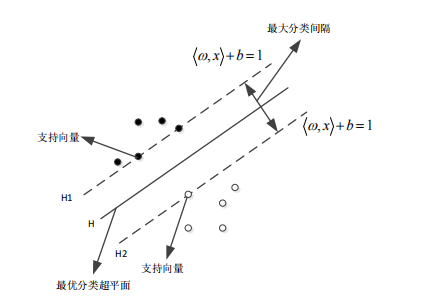
\includegraphics[width=0.5\textwidth]{svm.png}
        \caption{SVM模型原理图}
        \label{fig:svm}
    \end{figure}

    2、表模板
    \begin{table}[htpb]
        \caption{最优算法的多指标分析}
        \begin{center}\label{table:score}
            \begin{tabular}{|c|r|r|r|}
                \hline
                     & \multicolumn{1}{c|}{精确率} & \multicolumn{1}{c|}{召回率} & \multicolumn{1}{c|}{F1得分} \\ \hline
                石块 & 0.94                        & 0.96                        & 0.95                        \\ \hline
                金属 & 0.92                        & 0.97                        & 0.95                        \\ \hline
                塑料 & 0.96                        & 0.89                        & 0.93                        \\ \hline
            \end{tabular}
        \end{center}
    \end{table}

    3、公式模板
    \begin{equation}\label{eq:svmsuper}
        \begin{array}{l}
            \min _{\boldsymbol{w}, b} \frac{1}{2}\|\boldsymbol{w}\|^{2} \\
            \text { s.t. } y_{i}\left(\boldsymbol{w}^{\mathrm{T}} \boldsymbol{x}_{i}+b\right) \geqslant 1, \quad i=1,2, \ldots, m
        \end{array}
    \end{equation}


    4、伪代码模板
    \begin{algorithm}[H]
        \caption{ K近邻算法步骤}
        \begin{algorithmic}[1]
            \Require
            训练数据集;
            待预测数据;
            \Ensure
            预测数据的类别;
            \State 加载数据;
            \State 初始化K值;
            \State 计算预测样本与训练集中的每一个样本的距离;
            \State 将距离和索引添加到有序集合中;
            \State 对距离按从小到大排序方式对距离和索引的有序集合进行排序;
            \State 从排序的集合中选择前K条数据;
            \State 获得选的K条数据的标签;
            \State 计算每一种标签的样本数量;
            \Return
            数量最多的标签作为样本的预测值;
        \end{algorithmic}
    \end{algorithm}


    5、代码模板
    \lstset{language=Python}
    \begin{lstlisting}
#调整图片尺寸到统一大小,并扁平化为一维数据
def image_to_feature_vector(image, size=(128, 128)):

	return cv2.resize(image, size).flatten()

#提取图像在HSV颜色空间上的颜色直方图,将直方图扁平化,
#作为特征向量返回
def extract_color_histogram(image, bins=(32, 32, 32)):
	hsv = cv2.cvtColor(image, cv2.COLOR_BGR2HSV)
	hist = cv2.calcHist([hsv], [0, 1, 2], None, bins,
		[0, 180, 0, 256, 0, 256])
	if imutils.is_cv2():
		hist = cv2.normalize(hist)
	else:
		cv2.normalize(hist, hist)
	return hist.flatten()

\end{lstlisting}
\end{appendices}

\end{document}
